% !TEX program = pdflatex
% !TEX options = -synctex=1 -interaction=nonstopmode -file-line-error "%DOC%"
% 固体物理第十次作业
\documentclass[UTF8,10pt,a4paper]{article}
\usepackage{ctex}
% \catcode`\。=\active
% \newcommand{。}{.}
\newcommand{\CourseName}{固体物理}
\newcommand{\CourseCode}{PHYS1502}
\newcommand{\Semester}{2019-2020学年第二学期}
\newcommand{\ProjectName}{第十次作业}
\newcommand{\DueTimeType}{截止时间}
\newcommand{\DueTime}{2020. 5. 15(周五)17:00}
\newcommand{\StudentName}{陈稼霖}
\newcommand{\StudentID}{45875852}
\usepackage[vmargin=1in,hmargin=.5in]{geometry}
\usepackage{fancyhdr}
\usepackage{lastpage}
\usepackage{calc}
\pagestyle{fancy}
\fancyhf{}
\fancyhead[L]{\CourseName}
\fancyhead[C]{\ProjectName}
\fancyhead[R]{\StudentName}
\fancyfoot[R]{\thepage\ / \pageref{LastPage}}
\setlength\headheight{12pt}
\fancypagestyle{FirstPageStyle}{
    \fancyhf{}
    \fancyhead[L]{\CourseName\\
        \CourseCode\\
        \Semester}
    \fancyhead[C]{{\Huge\bfseries\ProjectName}\\
        \DueTimeType\ : \DueTime}
    \fancyhead[R]{姓名 : \makebox[\widthof{\StudentID}][s]{\StudentName}\\
        学号 : \StudentID\\
        成绩 : \underline{\makebox[\widthof{\StudentID}]{}}}
    \fancyfoot[R]{\thepage\ / \pageref{LastPage}}
    \setlength\headheight{36pt}
}
\usepackage{amsmath,amssymb,amsthm,bm}
\allowdisplaybreaks[4]
\newtheoremstyle{Problem}
{}
{}
{}
{}
{\bfseries}
{.}
{ }
{第\thmnumber{ #2}\thmname{ #1}\thmnote{ (#3)} 得分: \underline{\qquad\qquad}}
\theoremstyle{Problem}
\newtheorem{prob}{题}
\newtheoremstyle{Solution}
{}
{}
{}
{}
{\bfseries}
{:}
{ }
{\thmname{#1}}
\makeatletter
\def\@endtheorem{\qed\endtrivlist\@endpefalse}
\makeatother
\theoremstyle{Solution}
\newtheorem*{sol}{解}
\providecommand{\abs}[1]{\left\lvert#1\right\rvert}
\usepackage{graphicx}
\begin{document}
\thispagestyle{FirstPageStyle}
\begin{prob}[(15.1) $\ddagger$Nearly Free Electron Model]
    Consider an electron in a weak periodic potential in one dimension $V(x)=V(x+a)$. Write the periodic potential as
    \[
        V(x)=\sum_Ge^{iGx}V_G
    \]
    where the sum is over the reciprocal lattice $G=2\pi n/a$, and $V_G^*=V_{-G}$ assure that the potential $V(x)$ is real.
    \begin{enumerate}
        \item[(a)] Explain why for $k$ near to a Brillouin zone boundary (such as $k$ near $\pi/a$) the electron wave-function should be taken to be
        \[
            \psi=Ae^{ikx}+Be^{i(k+G)x}\tag{15.14}
        \]
        where $G$ is a reciprocal lattice vector such that $\abs{k}$ is close to $\abs{k+G}$.
        \item[(b)] For an electron of mass $m$ with $k$ exactly at a zone boundary, use the above form of the wavefunction to show that the eigenenergies at this wavevector are
        \[
            E=\frac{\hbar^2k^2}{2m}+V_0\pm\abs{V_G}
        \]
        where $G$ is chosen so $\abs{k}=\abs{k+G}$.
        \begin{itemize}
            \item[$\triangleright$] Give a qualitative explanation of why these two states are separated in energy by $2\abs{V_G}$.
            \item[$\triangleright$] Give a sketch (don't do a full calculation) of the energy as a function of $k$ in both the extended and the reduced zone schemes.
        \end{itemize}
        \item[(c)] $^*$ Now consider $k$ close to, but not exactly at, the zone boundary. Give an expression for the energy $E(k)$ correct to order $(\delta k)^2$ where $\delta k$ is the wavevector difference from $k$ to the zone boundary wavevector.
        \begin{itemize}
            \item[$\triangleright$] Calculate the effective mass of electron at this wavevector.
        \end{itemize}
    \end{enumerate}
\end{prob}
\begin{sol}
    \begin{enumerate}
        \item[(a)] 因为在布里渊区边界处,波矢为$k$的电子和波矢为$k+G$的电子具有相近的能量,所以当使用微扰理论时,能量的二阶修正项的分母趋于$0$,此时必须采用简并微扰理论。在由$\vert k\rangle$和$\vert k+G\rangle$组成的子希尔伯特空间中,求解哈密顿矩阵
        \begin{align}
            H=\left(\begin{matrix}
                E_0&V_G\\
                V_G^*&E_0
            \end{matrix}\right)
        \end{align}
        的本征函数,就会得到其本征函数是两个波函数$\vert k\rangle=e^{ikx}$,$\vert k+G\rangle=e^{i(k+G)x}$的线性组合.
        \item[(b)] 
        \begin{itemize}
            \item[$\triangleright$] 定性的解释:在布里渊区边界处,状态$\vert k\rangle$和$\vert k+G\rangle$简并,周期性势场作为一种微扰存在,将这两个能级的简并去除了.\\
            定量的解释:本征态的能量可通过求解哈密顿的本征值得到. 在布里渊区边界处,电子的哈密顿矩阵的各个矩阵元为
            \begin{align}
                \langle k\rvert H\lvert k\rangle=&\frac{\hbar^2k^2}{2m}+V_0,\\
                \langle k+G\rvert H\lvert k+G\rangle=&\frac{\hbar^2(k+G)^2}{2m}+V_0,\\
                \langle k\rvert H\lvert k+G\rangle=&V_G,\\
                \langle k+G\rvert H\lvert k\rangle=&V_G^*.
            \end{align}
            因此哈密顿矩阵为
            \begin{align}
                H=\left(\begin{matrix}
                    \frac{\hbar^2k^2}{2m}+V_0&V_G\\
                    V_G^*&\frac{\hbar^2(k+G)^2}{2m}+V_0
                \end{matrix}\right)=\left(\begin{matrix}
                    \frac{\hbar^2}{2m}\left(-\frac{\pi}{a}\right)^2+V_0&V_G\\
                    V_G^*&\frac{\hbar^2}{2m}\left(\frac{\pi}{a}\right)^2
                \end{matrix}\right).
            \end{align}
            哈密顿矩阵的特征方程为
            \begin{align}
                \nonumber\lvert H-EI\rvert=&\left\lvert\begin{matrix}
                    \frac{\hbar^2}{2m}\left(-\frac{\pi}{a}\right)^2+V_0-E&V_G\\
                    V_G^*&\frac{\hbar^2}{2m}\left(\frac{\pi}{a}\right)^2+V_0-E
                \end{matrix}\right\rvert\\
                =&E^2-2\left[\frac{\hbar^2}{2m}\left(-\frac{\pi}{a}\right)^2+V_0\right]E+\left[\frac{\hbar^2}{2m}\left(\frac{\pi}{a}\right)^2+V_0\right]^2-\abs{V_G}^2=0.
            \end{align}
            解得哈密顿矩阵的本征值即为
            \begin{align}
                E=\frac{\hbar^2}{2m}\left(\frac{\pi}{a}\right)^2+V_0\pm\abs{V_G}.
            \end{align}
            \item[$\triangleright$] 简约布里渊区和拓展布里渊区的色散关系如图\ref{1-E-k}.
            \begin{figure}[h]
                \centering
                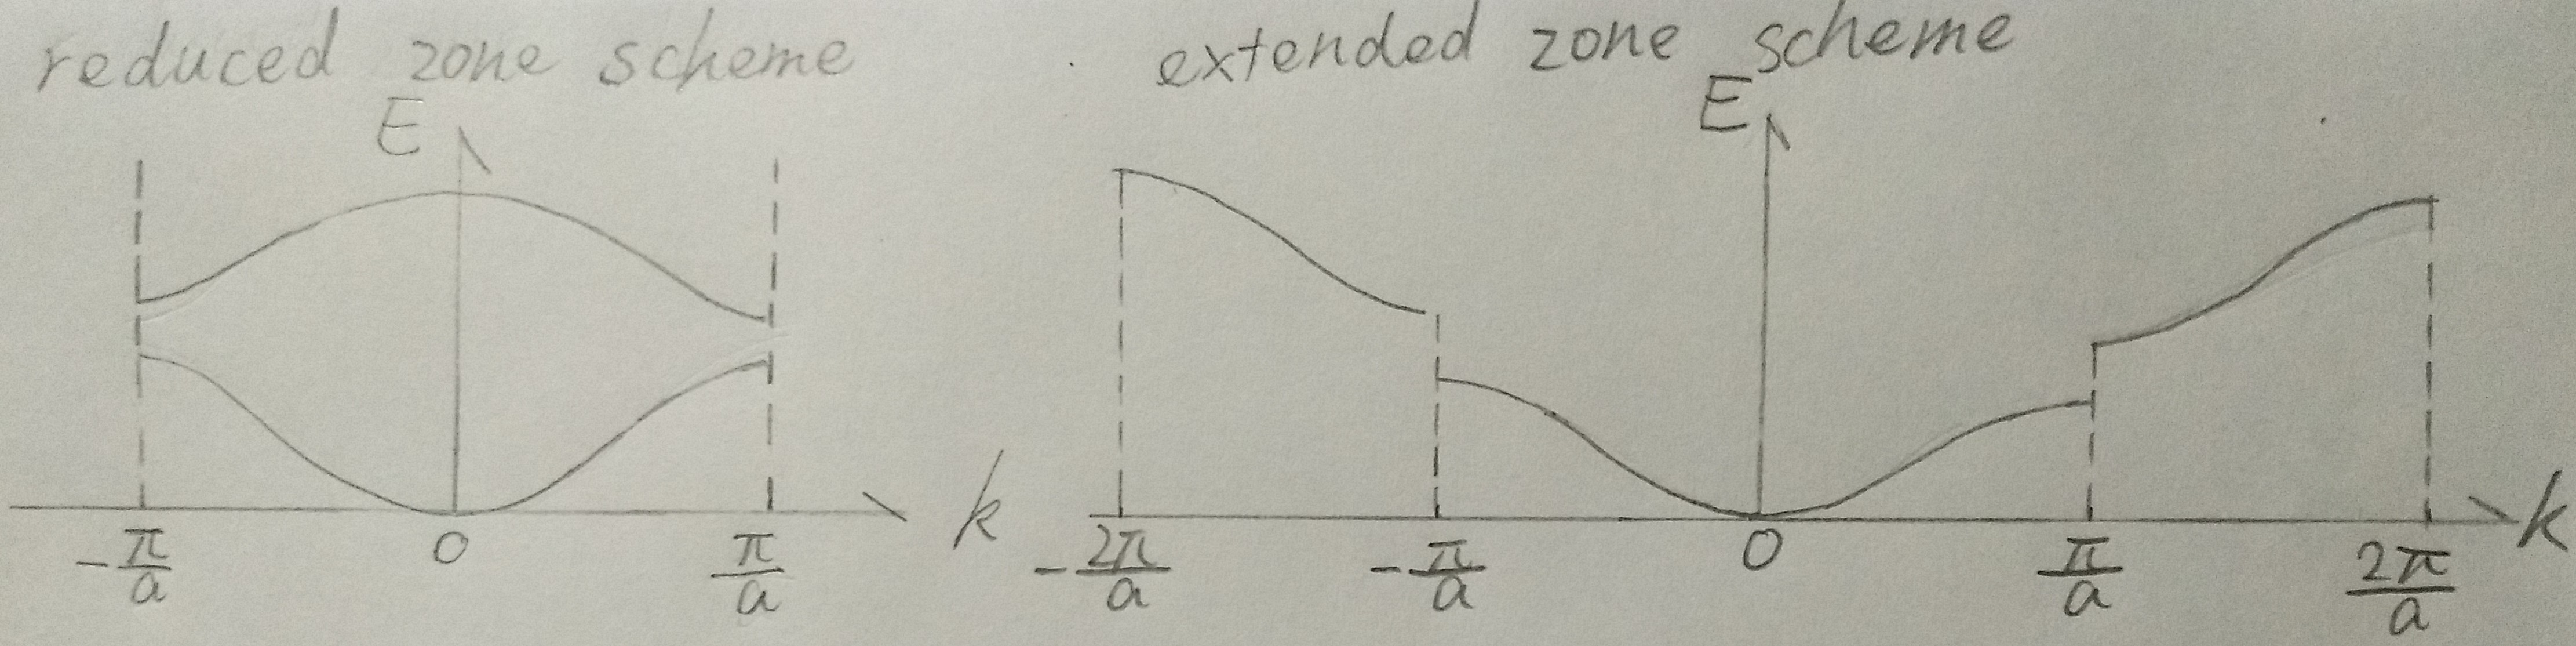
\includegraphics[width=.8\textwidth]{1-E-k.jpg}
                \caption{简约布里渊区和拓展布里渊区的色散关系.}
                \label{1-E-k}
            \end{figure}
        \end{itemize}
        \item[(c)] 当波矢$k$与布里渊区边界相差$\delta k$,哈密顿矩阵为
        \begin{align}
            H=\left(\begin{matrix}
                \frac{\hbar^2k^2}{2m}+V_0&V_G\\
                V_G^*&\frac{\hbar^2(k+G)^2}{2m}+V_0
            \end{matrix}\right)=\left(\begin{matrix}
                \frac{\hbar^2}{2m}\left(-\frac{\pi}{a}+\delta k\right)^2+V_0&V_G\\
                V_G^*&\frac{\hbar^2}{2m}\left(\frac{\pi}{a}+\delta k\right)^2+V_0
            \end{matrix}\right).
        \end{align}
        哈密顿矩阵的特征方程为
        \begin{align}
            \nonumber\abs{H-EI}=&\left\lvert\begin{matrix}
                \frac{\hbar^2}{2m}\left(-\frac{\pi}{a}+\delta k\right)^2+V_0-E&V_G\\
                V_G^*&\frac{\hbar^2}{2m}\left(\frac{\pi}{a}+\delta k\right)^2+V_0-E
            \end{matrix}\right\rvert\\
            \nonumber=&E^2+2\left\{\frac{\hbar^2}{2m}\left[\left(\frac{\pi}{a}\right)^2+(\delta k)^2\right]+V_0^2\right\}E\\
            &+\left\{\frac{\hbar^2}{2m}\left[\left(\frac{\pi}{a}\right)^2-2\left(\frac{\pi}{a}\right)\delta k+(\delta k)^2\right]+V_0\right\}\left\{\frac{\hbar^2}{2m}\left[\left(\frac{\pi}{a}\right)^2+2\left(\frac{\pi}{a}\right)\delta k+(\delta k)^2\right]+V_0\right\}-\abs{V_G}^2=0.\\
            \Longrightarrow&\left\{E-\frac{\hbar^2}{2m}\left[\left(\frac{\pi}{a}\right)^2+(\delta k)^2\right]-V_0\right\}^2=\left(\frac{\hbar^2}{2m}2\frac{\pi}{a}\delta k\right)^2+\abs{V_G}^2.
        \end{align}
        解得本征能量为
        \begin{align}
            E=\frac{\hbar^2}{2m}\left[\left(\frac{\pi}{a}\right)^2+(\delta k)^2\right]+V_0\pm\sqrt{\left(\frac{\hbar^2}{2m}2\frac{\pi}{a}\delta k\right)^2+\abs{V_G}^2}.
        \end{align}
        将上式做级数展开并保留到二阶项得
        \begin{align}
            \nonumber E=&\frac{\hbar^2}{2m}\left[\left(\frac{\pi}{a}\right)^2+(\delta k)^2\right]+V_0\pm\abs{V_G}\left[1\pm 2\left(\frac{\hbar^2}{2m}\frac{\pi}{a}\delta k\right)^2\right]\\
            =&\frac{\hbar^2}{2m}\left(\frac{\pi}{a}\right)^2+V_0\pm\abs{V_G}^2+\frac{\hbar^2}{2m}(\delta k)^2\left[1\pm\frac{\hbar^2}{m}\left(\frac{\pi}{a}\right)^2\frac{1}{\abs{V_G}}\right].
        \end{align}
        \begin{itemize}
            \item[$\triangleright$] 电子的有效质量为
            \begin{align}
                \nonumber m^*=&\frac{\hbar^2(\delta k)^2}{2E(\delta k)}=\frac{\hbar^2\left(\delta k\right)^2}{2\left\{\frac{\hbar^2}{2m}(\delta k)^2\left[1\pm\frac{\hbar^2}{m}\left(\frac{\pi}{a}\right)^2\frac{1}{\abs{V_G}}\right]\right\}}=m\left[1\pm\frac{\hbar^2}{m}\left(\frac{\pi}{a}\right)^2\frac{1}{\abs{V_G}}\right].
            \end{align}
        \end{itemize}
    \end{enumerate}
\end{sol}

\begin{prob}[(15.2) Periodic Functions]
    Consider a lattice of points $\{\bm{R}\}$ and a function $\rho(\bm{x})$ which has the periodicity of the lattice $\rho(\bm{x})=\rho(\bm{x}+\bm{R})$. Show that $\rho$ can be written as
    \[
        \rho(\bm{x})=\sum_{\bm{G}}\rho_{\bm{G}}e^{i\bm{G}\cdot\bm{x}}
    \]
    where the sum is over points $\bm{G}$ in the reciprocal lattice.
\end{prob}
\begin{sol}
    由函数$\rho(\bm{x})$的周期性,有
    \begin{align}
        \rho(\bm{x})=\frac{1}{N}\sum_{\bm{R}}\rho(\bm{x}+\bm{R}).
    \end{align}
    对$\rho(\bm{x}+\bm{R})$做傅里叶变换得
    \begin{align}
        \nonumber\rho(\bm{x})=&\frac{V}{N}\sum_{\bm{R}}\int\frac{d\bm{k}}{(2\pi)^3}\rho_{\bm{k}}e^{i\bm{k}\cdot(\bm{x}+\bm{R})}\\
        \nonumber=&\frac{V}{N}\int\frac{d\bm{k}}{(2\pi)^3}\rho_{\bm{k}}e^{i\bm{k}\cdot\bm{x}}\sum_{\bm{R}}e^{i\bm{k}\cdot\bm{R}}\\
        \nonumber=&\frac{V}{N}\int\frac{d\bm{k}}{(2\pi)^3}\rho_{k}e^{i\bm{k}\cdot\bm{x}}\frac{(2\pi)^3}{v}\sum_{\bm{G}}\delta^3(\bm{k}-\bm{G})\\
        =&\sum_{\bm{G}}\rho_{\bm{G}e^{i\bm{G}\cdot\bm{x}}}.
    \end{align}
\end{sol}

\begin{prob}[(15.3) Tight binding Bloch Wavfunctions]
    Analogous to the wavefunction introduced in Chapter 11, consider a tight-binding wave ansatz of the form
    \[
        \lvert\psi\rangle=\sum_{\bm{R}}e^{i\bm{k}\cdot\bm{R}}\lvert\bm{R}\rangle
    \]
    where the sum is over the points $\bm{R}$ of a lattice, and $\lvert\psi\rangle$ is the ground-state wavefunction of a electron bound to a nucleus on site $\bm{R}$. In real space this ansatz can be expressed as
    \[
        \psi(\bm{r})=\sum_{\bm{R}}e^{i\bm{k}\cdot\bm{R}}\varphi(\bm{r}-\bm{R}).
    \]
    Show that this wavefunction is of the form required by Bloch' theorem (i.e., show it is a modified plane wave).
\end{prob}
\begin{sol}
    上述的波函数可化为
    \begin{align}
        \psi(\bm{r})=e^{i\bm{k}\cdot\bm{r}}\sum_{\bm{R}}e^{i\bm{k}\cdot(\bm{R}-\bm{r})}\varphi(\bm{r}-\bm{R})=e^{i\bm{k}\cdot\bm{r}}u(\bm{r}),
    \end{align}
    其中
    \begin{align}
        u(\vec{r})\equiv\sum_{\bm{R}}e^{i\bm{k}\cdot(\bm{R}-\bm{r})}\varphi(\bm{r}-\bm{R}).
    \end{align}
    因为当将$\bm{r}$平移一个晶格基矢,$\bm{r}\rightarrow\bm{r}+\bm{a}$
    \begin{align}
        u(\vec{r}+\bm{a})=\sum_{\bm{R}}e^{i\bm{k}\cdot[(\bm{R}-\bm{a})-\bm{r}]}\varphi(\bm{r}-(\bm{R}-\bm{a}))=\sum_{\bm{R}-\bm{a}}e^{i\bm{k}\cdot(\bm{R}-\bm{r})}\varphi(\bm{r}-\bm{R}),
    \end{align}
    根据平移群的性质,将群内的所有矢量与一个晶格基矢相减,得到的仍然是原先的平移群,$\bm{R}-\bm{a}\rightarrow\bm{R}$,故
    \begin{align}
        u(\vec{r}+\bm{a})=\sum_{\bm{R}}e^{i\bm{k}\cdot(\bm{R}-\bm{r})}\varphi(\bm{r}-\bm{R})=u(\vec{r}),
    \end{align}
    $u(\vec{r})$是一个以$\bm{a}$为周期的周期函数,故$\psi(\bm{r})$满足布洛赫定理要求的形式.
\end{sol}

\begin{prob}[(15.4) $^*$Nearly Free Electrons in Two Dimensions]
    Consider the nearly free electron model for a square lattice with lattice constant $a$. Suppose the periodic potential is given by
    \begin{align*}
        V(x,y)&=2V_{10}[\cos(2\pi x/a)+\cos(2\pi y/a)]\\
        &+4V_{11}[\cos(2\pi x/a)\cos(2\pi y/a)]
    \end{align*}
    \begin{enumerate}
        \item[(a)] Use the nearly free electron model to find the energies of states at wavevector $\bm{G}=(\pi/a,0)$.
        \item[(b)] Calculate the energies of the states at wavevector $\bm{G}=(\pi/a,\pi/a)$. (Hint: You should write down a $4$ by $4$ secular determinant, which looks difficult, but a actually factors nicely. Make use of adding together rows or columns of the determinant before trying to evaluate it!)
    \end{enumerate}
\end{prob}
\begin{sol}
    \begin{enumerate}
        \item[(a)] $\bm{G}$处于$x$方向上的布里渊区边界,$y$方向上的布里渊区中心,故其能量应当等于一维周期势场中布里渊区边界处的能量,其能量应为
        \begin{align}
            E=\frac{\hbar^2}{2m}\left(\frac{\pi}{a}\right)^2\pm\abs{V_{\bm{G}}},
        \end{align}
        其中
        \begin{align}
            \label{4-ME}
            \nonumber\abs{V_{\bm{G}}}=&\abs{\langle(-\pi/a,0)\rvert V(x,y)\lvert(\pi/a,0)\rangle}\\
            \nonumber=&\abs{\frac{1}{a^2}\int_{-a/2}^{a/2}dx\int_{-a/2}^{a/2}dy\,(e^{-i\pi x/a})^*\{2V_{10}[\cos(2\pi x/a)+\cos(2\pi y/a)]+4V_{11}[\cos(2\pi x/a)\cos(2\pi y/a)]\}e^{i\pi x/a}}\\
            =&\abs{V_{10}}.
        \end{align}
        \item[(b)] 状态$\lvert(\pi/a,\pi/a)\rangle$和状态$\lvert(\pi/a,-\pi/a)\rangle,\lvert(-\pi/a,-\pi/a)\rangle,\lvert(-\pi/a,\pi/a)\rangle$简并,在以这四个状态依次为基矢组成的子希尔伯特空间中,如式\ref{4-ME}那样,用
        \begin{align}
            H_{i,j}=\langle \psi_i\rvert H\lvert \psi_j\rangle
        \end{align}
        我们可以算出哈密顿矩阵的各个矩阵元,从而得到哈密顿矩阵为
        \begin{align}
            H=\left(\begin{matrix}
                \varepsilon&V_{10}&V_{11}&V_{10}\\
                V_{10}&\varepsilon&V_{10}&V_{11}\\
                V_{11}&V_{10}&\varepsilon&V_{10}\\
                V_{10}&V_{11}&V_{10}&\varepsilon
            \end{matrix}\right),
        \end{align}
        其中$\varepsilon=\frac{\hbar^2}{2m}\left[\left(\frac{\pi}{a}\right)^2+\left(\frac{\pi}{a}\right)^2\right]$为自由电子的能量.
        这一哈密顿矩阵的特征方程为
        \begin{align}
            \abs{H-EI}=\left\lvert\begin{matrix}
                \varepsilon-E&V_{10}&V_{11}&V_{10}\\
                V_{10}&\varepsilon-E&V_{10}&V_{11}\\
                V_{11}&V_{10}&\varepsilon-E&V_{10}\\
                V_{10}&V_{11}&V_{10}&\varepsilon-E
            \end{matrix}\right\rvert=0.
        \end{align}
        对这一行列式做如下操作:用第一行减去第三行,用第二行减去第四行,得到
        \begin{align}
            \left\lvert\begin{matrix}
                \varepsilon-E-V_{11}&0&V_{11}-\varepsilon+E&0\\
                0&\varepsilon-E-V_{11}&0&V_{11}-\varepsilon+E\\
                V_{11}&V_{10}&\varepsilon-E&V_{10}\\
                V_{10}&V_{11}&V_{10}&\varepsilon-E
            \end{matrix}\right\rvert=0.
        \end{align}
        然后再将第三列加到第一列,将第四列加到第二列,得到
        \begin{align}
            \nonumber&\left\lvert\begin{matrix}
                0&0&V_{11}-\varepsilon+E&0\\
                0&0&0&V_{11}-\varepsilon+E\\
                \varepsilon-E+V_{11}&2V_{10}&\varepsilon-E&V_{10}\\
                2V_{10}&\varepsilon-E+V_{11}&V_{10}&\varepsilon-E
            \end{matrix}\right\rvert\\
            =&(V_{11}-\varepsilon+E)^2[(\varepsilon-E+V_{11})^2-4V_{10}^2]=0.
        \end{align}
        解得本征能量为
        \begin{align}
            E_1=E_2=\varepsilon-V_{11},\quad E_3=\varepsilon+V_{11}-2V_{10},\quad E_4=\varepsilon+V_{11}+2V_{10}.
        \end{align}
    \end{enumerate}
\end{sol}

\begin{prob}[(15.6) Kronig-Penney Model$^*$]
    Consider electrons of mass $m$ in a so-called "delta-function comb" potential in one dimension
    \[
        V(x)=aU\sum_n\delta(x-na)
    \]
    \begin{enumerate}
        \item[(a)] Argue using the Schrodinger equation that in-between delta functions, an eigenstate of energy $E$ is always of a plane wave form $e^{iq_Ex}$ with
        \[
            q_E=\sqrt{2mE}/\hbar.
        \]
        Using Bloch's theorem conclude that we can write an eigenstate with energy $E$ as
        \[
            \psi(x)=e^{ikx}u_E(x)
        \]
        where $u(E)$ is a periodic function defined as
        \[
            u_E(x)=A\sin(q_Ex)+B\cos(q_Ex)\quad 0<x<a
        \]
        and $u_E(x)=u_E(x+a)$ defines $u$ outside of this interval.
        \item[(b)] Using continuity of the wavefunction at $x=0$ derive
        \[
            B=e^{-ika}[A\sin(q_Ea)+B\cos(q_Ea)],
        \]
        and using the Schrodinger equation to fix the discontinuity in slope at $x=0$ derive
        \[
            q_EA-e^{ikx}q_E[A\cos(q_Ea)-B\sin(q_Ea)]=2maUB/\hbar^2
        \]
        Solve these two equations to obtain
        \[
            \cos(ka)=\cos(q_Ea)+\frac{mUa}{\hbar^2q_E}\sin(q_Ea)
        \]
        The left-hand side of this equation is always between $-1$ and $1$, but the right-hand side is not. Conclude that there must be values of $E$ for which there are no solutions of the Schrodinger equation --- hence concluding there are gap in the spectrum.
        \item[(c)] For small values of the potential $U$ show that this result agrees with the prediction of the nearly free electron model (i.e., determine the size of the gap at the zone boundary).
    \end{enumerate}
\end{prob}
\begin{sol}
    \begin{enumerate}
        \item[(a)] 在两个delta势之间,由于势能为$0$,所以薛定谔方程为
        \begin{align}
            -\frac{\hbar^2}{2m}\frac{d^2}{dx^2}\psi(x)=E,
        \end{align}
        这是典型的波动方程的形式,其波函数必为平面波的形式:
        \begin{align}
            \psi(x)=\alpha e^{iq_Ex}+\beta e^{-iq_Ex}=A\sin(q_Ex)+B\cos(q_Ex).
        \end{align}
        其中$q_E=\sqrt{2mE}/\hbar$.
        根据布洛赫定理,波函数可化为这样的形式
        \begin{align}
            \psi(x)=e^{ikx}u_E(x),
        \end{align}
        其中$u_E(x)$是以$a$为周期的函数. 故
        \begin{align}
            \psi(x+a)=e^{ik(x+a)}u_E(x+a)=e^{ik(x+a)}u_E(x)=e^{ika}\psi(x).
        \end{align}
        且$u_E(x)$也具有如下的形式:
        \begin{align}
            u_E(x)=\frac{\psi(x)}{e^{ikx}}=\alpha e^{i(q_E-k)x}+\beta e^{-i(q_E+k)x}=A'\sin((q_E-k)x)+B'\cos((q_E-k)x).
        \end{align}
        \item[(b)] 根据$u$的周期性,其在$x=0$处的函数值应当等于在$x=a$处的函数值
        \begin{align}
            u_E(0)=B=u_E(a)=e^{-ika}[A\sin(q_Ea)+B\cos(q_Ea)].
        \end{align}
        波函数的导数为
        \begin{align}
            \label{5-1}
            \psi(x)=Aq_E\cos(q_Ex)-Bq_E\sin(q_Ex).
        \end{align}
        在$x=0$处对薛定谔方程两边关于$x$进行积分,得到
        \begin{align}
            \nonumber\int_{0^-}^{0^+}dx\,\frac{\hbar^2}{2m}\frac{d^2}{dx^2}\psi(x)=&-\frac{\hbar^2}{2m}[\psi'(0^+)-\psi'(0^-)]=-\frac{\hbar^2}{2m}[\psi'(0^+)-e^{-ika}\psi'(a^-)]\\
            \nonumber=&-\frac{\hbar^2}{2m}[Aq_E-e^{-ika}(Aq_E\cos(q_Ea)-Bq_E\sin(q_Ea))]\\
            =&\int_{0^-}^{0^+}aU\sum_n\delta(x-na)\psi(x)\,dx\\
			=&aUB.
        \end{align}
        \begin{align}
            \label{5-2}
            \Longrightarrow q_EA-e^{-ika}q_E[A\cos(q_Ea)-B\sin(q_Ea)]=-\frac{2maUB}{\hbar^2}.
        \end{align}
        将式\ref{5-1}代入式\ref{5-2},消去$A$和$B$,可得
        \begin{align}
            \cos(ka)=\cos(q_Ea)+\frac{mUa}{\hbar^2q_E}\sin(q_Ea).
        \end{align}
        上式左侧的取值范围为$[-1,1]$,而右侧则可能在这一范围之外,因此当$E$取某些值时,薛定谔方程无解而产生带隙.
        \item[(c)] 在布里渊区边界$k=\frac{\pi}{a}$附近,$q_E\approx k+\delta$,上式化为
        \begin{gather}
            -1=\cos(\pi+\delta a)+\frac{mUa}{\hbar^2(\frac{\pi}{a}+\delta)}\sin(\pi+\delta a).
        \end{gather}
        上式右边关于$\delta$展开并保留到二阶项,得
        \begin{gather}
            -1=-1+\frac{1}{2}(\delta a)^2-\frac{mUa}{\hbar^2\pi}(1+\frac{\delta a}{\pi})\delta a,\\
            \Longrightarrow\delta=0\text{或}\approx\frac{2mUa}{\hbar^2\pi}.
        \end{gather}
        电子的能量为
        \begin{align}
            E=\frac{\hbar^2}{2m}\left(\frac{\pi}{a}+\delta\right)^2\approx E_0\text{或}\approx E_0+2U_0.
        \end{align}
        其中
        \begin{align}
            V_G=\frac{1}{a}\int_{-a/2}^{a/2}dx\,e^{-iGx}V(x)e^{iGx}=U.
        \end{align}
        带隙$2\abs{U}=2\abs{V_G}$与用进自由电子计算得到的一致.
    \end{enumerate}
\end{sol}
\end{document}